\section{Undecidability of the A-TSO game}
\label{apx:atso}

In this section, we will formally prove the correctness of the reduction presented in \autoref{sec:group-III}.
We begin with the construction of the TSO program $\program = \tuple{\process^1, \process^2, \process^3}$.
For $\process^1$, we start by adding the states of $\channelstateset$ to $\stateset^1$.
Then, for each transition of $\channelsystem$, we add some auxiliary states $\hstate_1, \hstate_2, \dots$ and transitions between them to simulate the PCS behaviour.
\autoref{fig:a-reduction-1} shows this construction for each of the transitions $\channelstate \to[\nop] \channelstate'$, $\channelstate \to[!\channelmessage] \channelstate'$ and $\channelstate \to[?\channelmessage] \channelstate'$.
Note that all the auxiliary states of $\process^1$ (labelled as $\hstate_i$) are supposed to be distinct for each transition.

Additionally, \autoref{fig:a-reduction-2} and \autoref{fig:a-reduction-3} show the process definitions of $\process^2$ and $\process^3$, respectively.
The set of final states is $\stateset_F^\program := \channelstateset_F \cup \set{ \state_F, \rstate_F }$, where $\channelstateset_F \subset \stateset^1$, $\state_F \in \stateset^2$ and $\rstate_F \in \stateset^3$.

\begin{figure}
\centering

% skip
\begin{subfigure}[b]{0.45\linewidth}
\centering
\begin{tikzpicture}[
    state/.style={},
    xscale=1,yscale=-1
]
    \node[state]	at (0,0)	(q1) {$\channelstate$};
    \node[state]	at (0,1)	(h1) {$\hstate_1$};
    \node[state]	at (0,2)	(q2) {$\channelstate'$};

    \draw[->] (q1) -- node[right] {$\nop$} (h1);
    \draw[->] (h1) -- node[right] {$\nop$} (q2);
\end{tikzpicture}
\bigskip
\caption{skip operation $\channelstate \to[\nop] \channelstate'$}
\end{subfigure}
\hfill
%
% send
\begin{subfigure}[b]{0.45\linewidth}
\centering
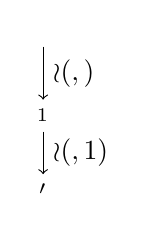
\begin{tikzpicture}[
    state/.style={},
    xscale=1,yscale=-1
]
    \node[state]	at (0,0)	(q1) {$\channelstate$};
    \node[state]	at (0,1)	(h1) {$\hstate_1$};
    \node[state]	at (0,2)	(q2) {$\channelstate'$};

    \draw[->] (q1) -- node[right] {$\wr(\xwr,\channelmessage)$} (h1);
    \draw[->] (h1) -- node[right] {$\wr(\yvar,1)$} (q2);
\end{tikzpicture}
\bigskip
\caption{send operation $\channelstate \to[!\channelmessage] \channelstate'$}
\end{subfigure}

\bigskip
\bigskip

% receive
\begin{subfigure}{\linewidth}
\centering
\begin{tikzpicture}[
    state/.style={},
    xscale=1,yscale=-1
]
    \node[state]	at (0,0)	(q1) {$\channelstate$};
    \node[state]	at (0,1)	(h1) {$\hstate_1$};
    \node[state]	at (0,2)	(h2) {$\hstate_2$};
    \node[state]	at (0,3)	(h3) {$\hstate_3$};
    \node[state]	at (0,4)	(q2) {$\channelstate'$};

    \node[state]	at (4,1)	(h4) {$\hstate_4$};
    \node[state]	at (4,2)	(h5) {$\hstate_5$};
    \node[state]	at (4,3)	(h6) {$\hstate_6$};

    \draw[->] (q1) -- node[right] {$\nop$} (h1);
    \draw[->] (h1) -- node[right] {$\rd(\xrd,\channelmessage)$} (h2);
    \draw[->] (h2) -- node[right] {$\rd(\xrd,\bot)$} (h3);
    \draw[->] (h3) -- node[right] {$\nop$} (q2);

    \draw[->] (h1) -- node[above] {$\mf$} (h4);
    \draw[->] (h4) -- node[right] {$\nop$} (h5);
    \draw[->] (h5) -- node[right] {$\rd(\xwr,\bot)$} (h6);
\end{tikzpicture}
\bigskip
\caption{receive operation $\channelstate \to[?\channelmessage] \channelstate'$}
\end{subfigure}

\caption{$\process^1$ of the A-TSO reduction from PCS}
\label{fig:a-reduction-1}
\end{figure}

\begin{figure}
\centering
\begin{tikzpicture}[
    state/.style={},
    xscale=1,yscale=-1
]
    \node[state] at (0,0) (q1) {$\state_1$};
    \node[state] at (0,1) (q2) {$\state_\channelmessage$};
    \node[state] at (0,2) (q3) {$\state_3$};
    \node[state] at (0,3) (q4) {$\state_4$};
    \node[state] at (0,4) (q5) {$\state_5$};
    \node[state] at (0,5) (q6) {$\state_6$};
    \node[state] at (0,6) (q7) {$\state_7$};
    \node[state] at (0,7) (q8) {$\state_8$};
    \node[state] at (0,8) (q9) {$\state_9$};
    \node[state] at (0,9) (q10) {$\state_{10}$};
    \node[state] at (0,10) (q1') {$\state_1$};

    \draw[->] (q1) -- node[right] {$\rd(\xwr,\channelmessage)$} (q2);
    \draw[->] (q2) -- node[right] {$\wr(\xrd,\channelmessage)$} (q3);
    \draw[->] (q3) -- node[right] {$\wr(\xwr,\bot)$} (q4);
    \draw[->] (q4) -- node[right] {$\mf$} (q5);
    \draw[->] (q5) -- node[right] {$\nop$} (q6);
    \draw[->] (q6) -- node[right] {$\rd(\yvar,1)$} (q7);
    \draw[->] (q7) -- node[right] {$\wr(\yvar,0)$} (q8);
    \draw[->] (q8) -- node[right] {$\mf$} (q9);
    \draw[->] (q9) -- node[right] {$\wr(\xrd,\bot)$} (q10);
    \draw[->] (q10) -- node[right] {$\mf$} (q1');

    \node[state] at (5,0) (qf) {$\state_F$};
    \draw[->] (q1) -- node[above right] {$\rd(\xwr,\channelmessage)$} (qf);

    \node[state] at (5,2) (qf) {$\state_F$};
    \draw[->] (q3) -- node[above right] {$\rd(\yvar,1)$} (qf);

    \node[state] at (5,3) (qf) {$\state_F$};
    \draw[->] (q4) -- node[above right] {$\nop$} (qf);

    \node[state] at (5,4) (qf) {$\state_F$};
    \draw[->] (q5) -- node[above right] {$\rd(\yvar,1)$} (qf);

    \node[state] at (5,8) (qf) {$\state_F$};
    \draw[->] (q9) -- node[above right] {$\rd(\xwr,\channelmessage)$} (qf);

    \draw[thick,decoration={brace, mirror},decorate] (q1.south west) -- node[left]{for all $\channelmessage \in \channelmessageset$} (q3.north west);
\end{tikzpicture}
\bigskip
\caption{$\process^2$ of the A-TSO reduction from PCS}
\label{fig:a-reduction-2}
\end{figure}

\begin{figure}
\centering
\begin{tikzpicture}[
    state/.style={},
    xscale=1,yscale=-1
]
    \node[state] at (0,0) (q1) {$\rstate_1$};
    \node[state] at (0,1) (q2) {$\rstate_2$};
    \node[state] at (-2,2) (q3) {$\rstate_3$};
    \node[state] at (2,2) (qf) {$\rstate_F$};

    \draw[->] (q1) -- node[right] {$\nop$} (q2);
    \draw[->] (q2) -- node[above left] {$\nop$} (q3);
    \draw[->] (q2) -- node[above right] {$\nop$} (qf);
    \draw[->] (q3) to[out=45,in=135,loop] node[below] {$\nop$} (q3);
    \draw[->] (qf) to[out=45,in=135,loop] node[below] {$\nop$} (qf);
\end{tikzpicture}
\bigskip
\caption{$\process^3$ of the A-TSO reduction from PCS}
\label{fig:a-reduction-3}
\end{figure}


\begin{thm}
\label{thm:equivalence-atso-pcs}
    Consider the A-TSO game, where player A can update the buffer before and after her turn, but player B can never update.
    The set of final states $\channelstateset_F$ of $\channelsystem$ is reachable from $\channelstate_0 \in \channelstateset$ if and only if player B wins the game $\game^\TSO(\program, \stateset_F^\program)$ starting from the configuration $\conf_0 := \tuple{ \tuple{\channelstate_0, \state_1, \rstate_1}, \tuple{\varepsilon, \varepsilon, \varepsilon}, \set{ \xwr \mapsto \bot, \xrd \mapsto \bot, \yvar \mapsto 0} }_B \in \confset_B$.
\end{thm}

Note that the definition of $\process^3$ secures deadlock-freedom of $\program$.
Furthermore, if one of the players has no enabled transitions in either $\process^1$ or $\process^2$ in her turn, she will lose the game:
If player A has no enabled transition, she needs to move from $\rstate_1$ to $\rstate_2$ in $\process^3$.
Player B can then respond with $\rstate_2 \to \rstate_3 \in \stateset_F^\program$, which player A cannot escape from.
Similarly, if player B needs to move to $\rstate_2$, player A can respond with $\rstate_4$.
Since player A controls the buffer updates, she can decide to not perform any buffer updates, which maintains the situation that player B can only move in $\process^3$.
Thus, the game will loop in $\rstate_4 \to \rstate_4$ forever, which means that player A wins.

In the following, we say that a player is \emph{deadlocked}, if it is her turn and there is no enabled outgoing transition in either $\process^1$ or $\process^2$.
Naturally, both players avoid being deadlocked, since it means that they lose the game, respectively.

\subsection{From $\channelsystem$-Reachability to a Winning Strategy in A-TSO}

Suppose $\channelstateset_F$ is reachable from $\channelstate_0$.
Let $\conf_0^\channelsystem \to[\channeloperation_1]\ \conf_1^\channelsystem \to[\channeloperation_2]\ \dots \to[\channeloperation_n]\ \conf_n^\channelsystem$ be a run with $\conf_k^\channelsystem = \tuple{ \channelstate_k, \word_k }$ for all $k = 1, \dots, n$ and $s_n \in \channelstateset_F$.
Here, $\word_k$ is a word over $\channelmessageset$ consisting of the letters $\word_k[1], \dots, \word_k[\sizeof{\word_k}]$.
Without loss of generality we can assume that this run does not contain any duplicate configurations.

For all $k = 0, \dots, n$, we define a game configuration $\conf_k = \tuple{ \statemap_k, \buffermap_k, \memorymap_k }_B \in \confset_B$:
\begin{enumerate}
    \item\ $\statemap_k := \tuple{ \channelstate_k, \state_1, \rstate_1 }$
    \item\ $\buffermap_k := \tuple{ \tuple{\tuple{\yvar,1}, \tuple{\xwr,\word_k[1]}, \dots, \tuple{\yvar,1}, \tuple{\xwr,\word_k[\sizeof{\word_k}]}}, \varepsilon, \varepsilon }$
    \item\ $\memorymap_k := \set{ \xwr \mapsto \bot, \xrd \mapsto \bot, \yvar \mapsto 0 }$
\end{enumerate}
The basic idea is to develop a strategy for player B that visits all configurations $\conf_1, \dots, \conf_n$.
Inspecting the construction of $\process^2$, we observe that there is no way to prevent player A from performing the buffer update and rotation of the oldest channel message whenever she decides to do so.
We account for that by introducing additional configurations $c_k' = \tuple{ \statemap_k', \buffermap_k', \memorymap_k' }_B$:
\begin{enumerate}
    \item\ $\statemap_k' := \tuple{ \channelstate_k, \state_3, \rstate_1 }$
    \item\ $\buffermap_k' := \tuple{ \tuple{\tuple{\yvar,1}, \tuple{\xwr,\word_k[1]}, \dots, \tuple{\yvar,1}, \tuple{\xwr,\word_k[\sizeof{\word_k}-1]}, \tuple{\yvar,1}}, \varepsilon, \varepsilon }$
    \item\ $\memorymap_k^{(3)} := \set{ \xwr \mapsto \word_k[\sizeof{\word_k}], \xrd \mapsto \word_k[\sizeof{\word_k}], \yvar \mapsto 0 }$
\end{enumerate}
The configurations $\conf_k'$ refer to the case where player A has updated the oldest message to the memory and also performed the message rotation.
Note that if $\word_k = \varepsilon$, then $\conf_k'$ is not defined.

As a first step, consider a situation where it is player A's turn and $\process^2$ is in state $\state_1$.
If player A decides to initiate the message rotation by following the transition $\state_1 \to[\rd(\xwr,\channelmessage)] \state_\channelmessage$ for some $\channelmessage \in \channelmessageset$, we always let player B immediately respond with $\state_\channelmessage \to[\wr(\xrd,\channelmessage)] \state_3$.
On the other hand, if $\process^2$ is already in state $\state_3$, player A cannot take any further transitions in this process, since after $\state_3 \to[\wr(\xwr,\bot)] \state_4$, player B can take the transition $\state_4 \to[\nop] \state_F$ and wins.
We will use these observations in the following argumentation.

We show by induction that starting from $\conf_0$, Player B can force a play that either visits one of $\conf_k$, $\conf_k'$ or $\confset_F$.
For $k = 0$, this clearly holds true.
So, suppose that the claim holds for some arbitrary but fixed $0 \leq k < n$.
By the induction hypothesis, we can assume that the game is either in state $\conf_k$ or $\conf_k'$.

If $\channeloperation_{k+1} = \nop$, then player B takes the transition $\channelstate_k \to[\nop] \hstate_1$ in $\process^1$.
After a possible message rotation in $\process^2$ (i.e. one move by player A and B, respectively), player A is left with only one non-losing transition, which is $\hstate_1 \to[\nop] \channelstate_{k+1}$ in $\process^1$.
Assuming that player A can prevent an immediate defeat, we now need to show that the game is either in configuration $\conf_{k+1}$ or $\conf_{k+1}'$.

First, consider the case where $\process^2$ is in state $\state_1$, which implies that the sub-run started at $\conf_k$ rather than $\conf_k'$.
If player A had updated at least one message from the buffer to the memory, $\xwr$ would now contain some channel message $\channelmessage$.
Thus, player B could immediately win by taking the transition $\state_1 \to[\rd(\xwr,\channelmessage)] \state_F$.
We conclude that the game must be in configuration $\conf_{k+1}$.

In the other case, $\process^2$ is in state $\state_3$.
It follows that either the sub-run started in $\conf_k'$ or player A has updated a message from the buffer and performed the message rotation.
Suppose she had additionally updated at least one more message, in particular a message $\tuple{\yvar,1}$.
Then, player B is again able to win immediately by following $\state_3 \to[\rd(\yvar,1)] \state_F$.
Thus, the game must be in configuration $\conf_{k+1}'$.

Next, we examine the situation where $\channeloperation_{k+1} = {!}\channelmessage$, which is very similar to the previous one.
Player B takes the transition $\channelstate_k \to[\wr(\xwr,\channelmessage)] \hstate_1$ and player A eventually responds with $\hstate_1 \to[\wr(\yvar,1)] \channelstate_{k+1}$.
Using the same argumentation as above, either the game is now in configuration $\conf_{k+1}$ or $\conf_{k+1}'$, or player B can force an immediate win.

Lastly, if $\channeloperation_{k+1} = {?}\channelmessage$, player B starts by taking the transition $\channelstate_k \to[\nop] \hstate_1$ in $\process^1$.
For player A, $\hstate_1 \to[\mf] \hstate_4$ is losing:
Since $\channeloperation_{k+1} = {?}\channelmessage$, we know that $\word_k \neq \varepsilon$ and after flushing the buffer, the last character of $\word_k$ is written to $\xwr$.
Thus, after player B responds with $\hstate_4 \to[\nop] \hstate_5$, player A is effectively deadlocked, since the outgoing transition in $\process^1$ is disabled and all actions in $\process^2$ will eventually lead to player B reaching $\state_F$.

We conclude that player A updates and rotates the oldest message if not already done so, and then proceeds with $\hstate_1 \to[\rd(\xrd,\channelmessage)] \hstate_2$ in $\process^1$.
The only possible continuation for both players is now in $\process^2$:
$$ \state_3 \to[\wr(\xwr,\bot)] \state_4 \to[\mf] \state_5 \to[\nop] \state_6 \to[\rd(\yvar,1)] \state_7 \to[\wr(\yvar,0)] \state_8 \to[\mf] \state_9 \to[\wr(\xrd,\bot)] \state_{10} $$
Because of $\state_5 \to[\rd(\yvar,1)] \state_F$, player A cannot update the pending $\tuple{\yvar,1}$-message before reaching state $\state_6$, but then definitely has to do so to enable the next transition.
In $\state_9$, $\yvar$ is reset to $0$ again.
Furthermore, the transition $\state_9 \to[\rd(\xwr,\channelmessage)] \state_F$ ensures that no other message was updated.
When $\state_{10}$ is reached, player A needs to flush the buffer of $\process^2$ again, to enable both $\hstate_2 \to[\rd(\xrd,\bot)] \hstate_3$ in $\process^1$ and $\state_9 \to[\mf] \state_{10}$ in $\process^2$.
She then takes one of those two transitions and player B takes the other one.
Eventually (after maybe the update and rotation of the next message), player A will take the transition $\hstate_3 \to[\nop] \channelstate_{k+1}$ in $\process^1$.

At this point, $\process^1$ moved from $\channelstate_k$ to $\channelstate_{k+1}$ and $\process^2$ is back in $\state_1$ or $\state_3$.
Exactly one $\tuple{\yvar,1}$-message was removed from the buffer and the memory values of $\yvar$ and $\xrd$ were reset to $0$ and $\bot$, respectively.
Using the same argumentation as previously, we conclude that the game is now either in configuration $\conf_{k+1}$ or $\conf_{k+1}'$, or player B can force an immediate win.

This concludes the proof by induction.
In summary, starting from $\conf_0$, player B can force a play that reaches $\confset_B$ or one of the configurations $\conf_n$ or $\conf_n'$.
In both of these configurations, $\process^1$ is in the local state $\channelstate_n$, which is a final state of $\channelsystem$.
Thus, $\conf_n, \conf_n' \in \confset_B$ and player B wins in any case.

\subsection{From a Winning Strategy in A-TSO to $\channelsystem$-Reachability}

For the other direction, suppose that player B has a winning strategy.
Consider a strategy of player A that avoids reaching both $\state_F \in \stateset^2 \cap \stateset_F^\program$ and $\rstate_F \in \stateset^3 \cap \stateset_F^\program$ whenever possible.
Furthermore, assume that player A prefers to not update any messages and to move in $\process^2$, as long as it does not contradict the previous statement.

Let $\channelstate_0, \dots, \channelstate_n$ be the sequence of channel states that are visited by $\process^1$ during the run induced by these two strategies.
Since player B uses a winning strategy, this sequence is finite.
We will show by induction that for each $k = 0, \dots, n$, the run contains a game configuration $\conf_k = \tuple{ \statemap_k, \buffermap_k, \memorymap_k }_B \in \confset_B$ such that:
\begin{enumerate}
    \item\ $\statemap_k := \tuple{ \channelstate_k, \state_1, \rstate_1 }$
    \item\ $\buffermap_k := \tuple{ \tuple{\tuple{\yvar,1}, \tuple{\xwr,\word_k[1]}, \dots, \tuple{\yvar,1}, \tuple{\xwr,\word_k[\sizeof{\word_k}]}}, \varepsilon, \varepsilon }$, where $\word_k \in \channelmessageset\kstar$
    \item\ $\memorymap_k := \set{ \xwr \mapsto \bot, \xrd \mapsto \bot, \yvar \mapsto 0 }$
    \item\ If $k > 0$, there is a label $\channeloperation_k$ such that $\tuple{ \channelstate_{k-1}, \word_{k-1} } \to[\channeloperation_k]\ \tuple{ \channelstate_k, \word_k }$.
\end{enumerate}
For $k = 0$, this clearly holds true.
So, suppose that the claim holds for some arbitrary but fixed $0 \leq k < n$.

Starting in $\conf_k$, player B cannot move in $\process^2$, since $\memorymap(\xwr) = \bot$, $\buffermap(2) = \varepsilon$ and the only outgoing transitions from $\statemap(2) = \state_1$ are of the form $\rd(\xwr,\channelmessage)$ for $\channelmessage \in \channelmessageset$.
Thus, player B must first move in $\process^1$ instead.
Looking at the construction of $\process^1$, we see that the sub-run from $\conf_k$ to (the very next occurence of) $\channelstate_{k+1}$ takes a sequence of transitions that were added to $\program$ due to some unique transition $\channelstate_k \to[\channeloperation_{k+1}] \channelstate_{k+1}$ of $\channelsystem$.

If $\channeloperation_{k+1} = \nop$, we conclude that player B takes the transition $\channelstate_k \to[\nop]_\program \hstate_1$.
Player A has to respond with the only enabled transition in the resulting configuration, which is $\hstate_1 \to[\nop]_\program \channelstate_{{k+1}}$.
The game is now in a configuration with states $\stateset_k$, as defined above.
Furthermore, we conclude that the buffer must be $\buffermap_{k+1}$, where $\word_{k+1} := \word_k$, and the memory is $\memorymap_{k+1}$.
Finally, we have that $\tuple{ \channelstate_k, \word_k } \to[\nop] \tuple{ \channelstate_{k+1}, \word_{k+1} }$.
In other words, the game is now in position $\conf_k$.

If $\channeloperation_{k+1} = {!}\channelmessage$, we argue in the very same way as in the previous case that the run must have followed the transitions $\channelstate_k \to[\wr(\xwr,\channelmessage)]_\program \hstate_1 \to[\wr(\yvar,1)]_\program \channelstate_{k+11}$ in $\process^1$.
Similarly, the game is now in configuration $\conf_{k+1} = \tuple{ \statemap_{k+1}, \buffermap_{k+1}, \memorymap_{k+1} }_B$ with $\word_{k+1} := \channelmessage \bullet \word_k$.

Lastly, if $\channeloperation_{k+1} = {?}\channelmessage$, then player B takes $\channelstate_k \to[\nop]_\program \hstate_1$.
Assume that $\word_k = \varepsilon$, i.e. the buffer of $\process^1$ is empty.
Then, player A cannot update any message to the memory, which means that the transition $\hstate_1 \to[\mf]_\program \hstate_4$ is the only one that is enabled.
This leads to the path $\hstate_1 \to[\mf]_\program \hstate_4 \to[\nop]_\program \hstate_5 \to[\rd(\xwr,\bot)]_\program \hstate_6$, which ends in a deadlocked configuration for player B.
Since we already know that player B is winning, we conclude that the assumption was wrong and there is at least one pair of messages in the buffer of $\process^1$.

Thus, player A instead performs one buffer update of the oldest message $\tuple{\xwr, \channelmessage}$, where $\channelmessage$ is the last character of $\word_k$.
This enables $\state_1 \to[\rd(\xwr,\channelmessage)] \state_\channelmessage$ in $\process^2$, which player A executes.
Player B responds with $\state_\channelmessage \to[\wr(\xrd,\channelmessage)] \state_3$ in $\process^2$.
Player A immediately updates this message to the memory, which enables $\hstate_1 \to[\rd(\xrd,\channelmessage)] \hstate_2$ in $\process^1$, which she takes.
Note that this is her only choice since $\state_3 \to[\wr(\xwr,\bot)] \state_4$ opens up the possibility for player B to end the game by moving to $\state_F$.

Now, $\process^1$ is blocked again and the run continues in $\process^2$.
After
$$\state_3 \to[\wr(\xwr,\bot)] \state_4 \to[\mf] \state_5 \to[\nop] \state_6 \ ,$$
player A updates the oldest buffer message of $\process^1$, which is $\tuple{\yvar,1}$.
This is needed to enable
$$ \state_6 \to[\rd(\yvar,1)] \state_7 \to[\wr(\yvar,0)] \state_8 \to[\mf] \state_9 \to[\wr(\xrd,\bot)] \state_{10} \ .$$
Now, player A empties the buffer of $\process^2$ to execute the transition $\state_{10} \to[\mf] \state_1$.
This is followed by $\hstate_2 \to[\rd(\xrd,\bot)] \hstate_3 \to[\nop] \channelstate_{k+1}$ in $\process^1$.

We see that $\process^1$ is now in state $\channelstate_{k+1}$ and $\process^2$ is back in state $\state_1$, i.e. the process state is $\statemap_{k+1}$.
Since all memory values have also been reset to their default values, we conclude that the buffer state of the current game configuration is $\buffermap_{k+1}$, where $\word_{k+1} \bullet \channelmessage := \word_k$, and the memory is $\memorymap_{k+1}$.
Furthermore, the existence of the transition $\channelstate_k \to[?\channelmessage] \channelstate_{k+1}$ follows from the construction of $\program$, and it is enabled at the configuration $\tuple{\channelstate_k, \word_k}$ of $\channelsystem$, since $\channelmessage$ is the last character in $\word_k$.

This concludes the proof by induction.
In summary, we showed that $\channelsystem$ can reach the state $\channelstate_n$ starting from $\channelstate_0$.
What is left to show is that $\channelstate_n \in \channelstateset_F$.
Consider the continuation of the run after $\conf_n$.
If player B starts to simulate a skip or send operation, the run will inadvertedly visit another state of $\channelstateset$ after two moves, which is a contradiction, since we know that $\channelstate_n$ is the last such state that is visited.
Otherwise, if player B starts to simulate a receive operation, there are again two cases to consider.
If the buffer of $\process^1$ is empty, we have already seen that player A wins, which we know is not the case.
Otherwise, player A can just proceed as usually and continue to simulate the receive operation in $\process^1$ and $\process^2$.
In any case, player B has no opportunity to force the play into $\state_F$ or into a deadlock of player A.
In particular, player A can avoid to take $\state_3 \to[\nop] \state_4$, since there are exactly four (i.e. an even number of) moves to take before.

We conclude that the only way that player B wins the game is that $\channelstate_n \in \stateset_F^\program$, or $\channelstate_n \in \channelstateset_F$, equivalently.
Since $\channelstate_k \to \channelstate_{k+1}$ for all $k < n$, it follows that $\channelstateset_F$ is reachable from $\channelstate_0$.

\subsection{Proof of \autoref{thm:atso}}

This follows directly from \autoref{thm:equivalence-atso-pcs} and the undecidability of the state reachability problem for perfect channel systems \cite{DBLP:journals/jacm/BrandZ83}.

\subsection{Variants of A-TSO}

In the game where player A is restricted to perform updates only before her turn, one can check that the construction still works.
However, if player A is only allowed to update after her turn, we need to adjust the construction.
This is due to the fact that in the A-TSO game, there exist transitions where she is expected to update before her move.

We can easily fix this problem by adding two auxilliary states just before each of the affected transitions, and connect them with $\nop$ instructions.
This gives player A time to update the buffer after taking the auxiliary transition.

Furthermore, we add a transition from the second auxiliary state to a sink state, that is, a state with just a self-loop.
This prevents player B from taking the first transition, since player A can then go to the sink state, which effectively disables the process.
It also ensures that whenever player A takes the first auxiliary transition, player B has to respond by taking the second one.

We conclude that the modified construction gives rise to the same behaviour than the construction for A-TSO.
The formal proof is along the lines of \autoref{thm:equivalence-atso-pcs} or \autoref{thm:equivalence-btso-pcs}.
